\documentclass[12pt]{article}

% Packages
\usepackage[margin=1.2in]{geometry}
\usepackage{graphicx}
\usepackage{enumerate}
\usepackage{colortbl}
\usepackage{listings}
\usepackage{titling}
\usepackage{tabularx}
\usepackage{longtable}
\usepackage{booktabs}
\usepackage{hyperref}
\usepackage{makecell}
\usepackage{caption}
\usepackage{array}
\captionsetup[table]{skip=2pt}
% Comments --------------------------------------------------------------------
\usepackage{xcolor}
\newif\ifcomments\commentstrue
\ifcomments \newcommand{\authornote}[3]{\textcolor{#1}{[#3 ---#2]}}
\newcommand{\todo}[1]{\textcolor{red}{[TODO: #1]}} \else
\newcommand{\authornote}[3]{} \newcommand{\todo}[1]{} \fi
\newcommand{\wss}[1]{\authornote{magenta}{SS}{#1}}
\newcommand{\ds}[1]{\authornote{blue}{DS}{#1}}
% End Comments ---------------------------------------------------------------
\setlength{\parindent}{0pt}

% Title Page -----------------------------------------------------------------
\title{
\LARGE GEANT-4 GPU Port:
\\\vspace{10mm}
\large \textbf{Design Document: System Architecture}
\vspace{40mm}
}
\author{
\textbf{Team 8}
\\Stuart Douglas -- dougls2
\\Matthew Pagnan -- pagnanmm
\\Rob Gorrie -- gorrierw
\\Victor Reginato -- reginavp
\vspace{10mm}
}
\date{\vfill \textbf{System Architecture: Version 0}\\ \today}
% End Title Page -------------------------------------------------------------

% ============================== BEGIN DOCUMENT ============================= %
\begin{document}
\pagenumbering{gobble} % start numbering after TOC

% ============================== Title Page ============================= %
\maketitle
\newpage

% ================================= TOC ================================= %
\renewcommand{\contentsname}{Table of Contents}
\tableofcontents
\newpage
\pagenumbering{arabic}

\section{Introduction}% ============== Matt
\subsection{Revision History}
All major edits to this document will be recorded in the table below.

\begin{table}[h]
\centering
\caption{Revision History}\label{Table_Revision}
\begin{tabularx}{\textwidth}{Xll}
\toprule
\bf Description of Changes & \bf Author & \bf Date\\\midrule
Set up sections and filled out Introduction section & Matthew & 2015-12-15\\
\bottomrule
\end{tabularx}
\end{table}

\subsection{Terms Used}
\begin{table}[h]
\centering
\caption{Glossary}\label{Table_Glossary}
\begin{tabularx}{\textwidth}{lX}
\toprule
\bf Term & \bf Description\\\midrule\vspace{1mm}
Geant4 & open-source software toolkit for simulating particle interactions\\\vspace{1mm}
G4-STORK & fork of Geant4 developed by McMaster's Engineering Physics department to simulate McMaster's nuclear reactor\\\vspace{1mm}
GPU & graphics processing unit, well-suited to parallel computing tasks\\\vspace{1mm}
CPU & computer processing unit, well-suited to serial tasks\\\vspace{1mm}
CUDA & parallel computing architecture for GPU programming, developed by NVIDIA\\\vspace{1mm}
NVIDIA & computer hardware and software company specializing in GPU's\\
\bottomrule
\end{tabularx}
\end{table}

\subsection{List of Tables}
\begin{center}
\begin{tabular}{cl}
\toprule
\bf Table \# & \bf Title\\\midrule
\ref{Table_Revision} & Revision History\\
\ref{Table_Glossary} & Glossary\\
\ref{Table_RequirementsAndDesign} & Traceability of Requirements and Design\\
\bottomrule
\end{tabular}
\end{center}

\subsection{List of Figures}
\begin{center}
\begin{tabular}{cl}
\toprule
\bf Figure \# & \bf Title\\\midrule
\ref{imgUsesHierarchy} & Uses Hierarchy for G4NeutronHPVector\\
\bottomrule
\end{tabular}
\end{center}

\section{Overview}
\subsection{Purpose of Project}
The purpose of GEANT4-GPU is to reduce the computation times of particle simulations in Geant4 by parallelizing and running certain procedures on the GPU.

\subsection{Description}
The project aims to improve the computation times of Geant4 particle simulations by running certain parallel operations on a GPU. GEANT4-GPU will be a fork of the existing Geant4 system with the additional option for users with compatible hardware to run operations on the GPU for improved performane. This functionality will be available on Mac, Linux and Windows operating systems running on computers with NVIDIA graphics cards that support CUDA.\\

The design strategy for the project will be based on taking a specific, computationally heavy class from Geant4 and creating a class that fulfills the same interface but that runs on the GPU. This will be repeated for many classes until the project's deadline has been reached. The user will have the option of using the existing classes (running on the CPU) or the new ones (running on the GPU).

\subsection{Document Structure \& Template}
The design documentation for the project is based off of WHAT TEMPLATES?????? and is broken into two main documents.\\

This system architecture document details the system architecture, including an overview of the modules that make up the system, analysis of aspects that are likely and unlikely to change, reasoning behind the high-level decisions, and a table showing how each requirement is addressed in the proposed design.\\

A separate detailed design document covers the specifics of several key modules in the project. This includes the interface specification and implementation decisions.

\section{Important Design Decisions \& Reasoning}
\subsection{GPU Computing for Geant4}
GEANT4 simulations typically involve simulating the movement of billions of particles. These particles move independently of the other particles. Currently the particles are all stored in an array that the CPU has to go through moving each particle one by one. Considering how many particles this array holds this is a rather time consuming operation, especially since this movement of the particles is done often. 
Due to the nature of the particles being able to move independently of each other this is a problem that can be easily parallelized. Since the act of moving a particle is so simple GPU cores are able to execute these types of functions. So instead of parallelizing GEANT4 on multiple CPU's we can instead parallelize the code to run on all the GPU cores since the GPU has many more cores than the CPU it is able to run the parallelized code much faster.
\subsection{CUDA}
NVIDA recently created a toolkit to make creating parallel code on the GPU much easier. Due to how accessible and easy to use CUDA is to parallelize existing code CUDA was chosen to be as the architecture to be used for this project as it would require the least amount of understanding of the existing GEANT4 functions to produce speedups. 
\subsection{GPU Integration Approach}
\subsection{G4NeutronHPVector}\label{subsec_G4NeutronHPVector}
=======
\subsection{GPU Computing for Geant4} % matt
\subsection{CUDA} % matt
\subsection{GPU Integration Approach} % stu
When considering how to integrate the GPU computations with the non-ported procedures that run on the CPU there were several options. The first option would be to port the entire Geant4 toolkit to run 100\% on the GPU. This would see the biggest speedup, but is far beyond the scope of this project and the resources available. A more realistic alternative is to take several key classes and implement their functions on the GPU. The existing functions on the CPU would make the necessary calls to the GPU to execute the corresponding function and receive the result when the GPU finishes and return it to the caller. The advantage of this approach is that the work is easier to break down and distribute, and will focus efforts on the modules and functions within those modules that require speed improvements the most.\\

When a ported module is first initialized, it will also initialize a copy on the GPU, and every time data is updated those updates will be applied to the GPU class as well. Then, when a function is called, the GPU will already have all the data it requires and will be able to quickly return the result. If a given function is not ported or if the user has not enabled GPU computations the function will run the existing code on the CPU. The overhead of this approach is the time during initialization to initialize the GPU class as well, and when updates occur. We believe this overhead will be outweighed by the advantages of the parallel GPU computing. The initialization is only called once, and updates to the data generally target small subsets of the vector.\\

This same approach of taking a class and initializing a copy on the GPU with a subset of the functions ported to the GPU will be applied to other classes in the future.

\subsection{G4NeutronHPVector}\label{subsec_G4NeutronHPVector} % rob

\section{Likely and Unlikely Changes}

\subsection{Likely Changes} %========== Rob
\begin{enumerate}
\item
\end{enumerate}

\subsection{Unlikely Changes} %========= Rob
\begin{enumerate}
\item
\end{enumerate}

\subsection{Traceability of Likely Changes to Design Components}

\section{Module Hierarchy}%============= Stuart
\subsection{Decomposition of Components}
The project is based off of Geant4, an existing software system, and modifying specific modules of that system. As such, components do not need to be decomposed, instead the decomposition of the existing system will guide the modules in the project development.\\

Each module in Geant4 is represented by a C++ class, and the project will port a subset of said classes to the GPU. The decision of which classes to port to the GPU is derived from performance analysis of the program, with the most computationally time-consuming classes being the targets for GPU porting, such as G4NeutronHPVector as documented in section \ref{subsec_G4NeutronHPVector}.

\subsection{Uses Hierarchy}
Since each modified module of the project will have a direct 1-to-1 relationship with an existing module in Geant4, the uses hierarchy with the new, GPU-enabled classes will be identical to the existing uses hierarchy of Geant4 with their corresponding existing classes.\\

Geant4 is an extremely large system with many modules, so its entire uses hierarchy will not be documented here. Instead, the following hierarchy just maps the dependencies of G4NeutronHPVector, which is currently the focus of the project. Note that modules used by system libraries are not included.
\begin{figure}
\caption{Uses Hierarchy for G4NeutronHPVector}\label{imgUsesHierarchy}
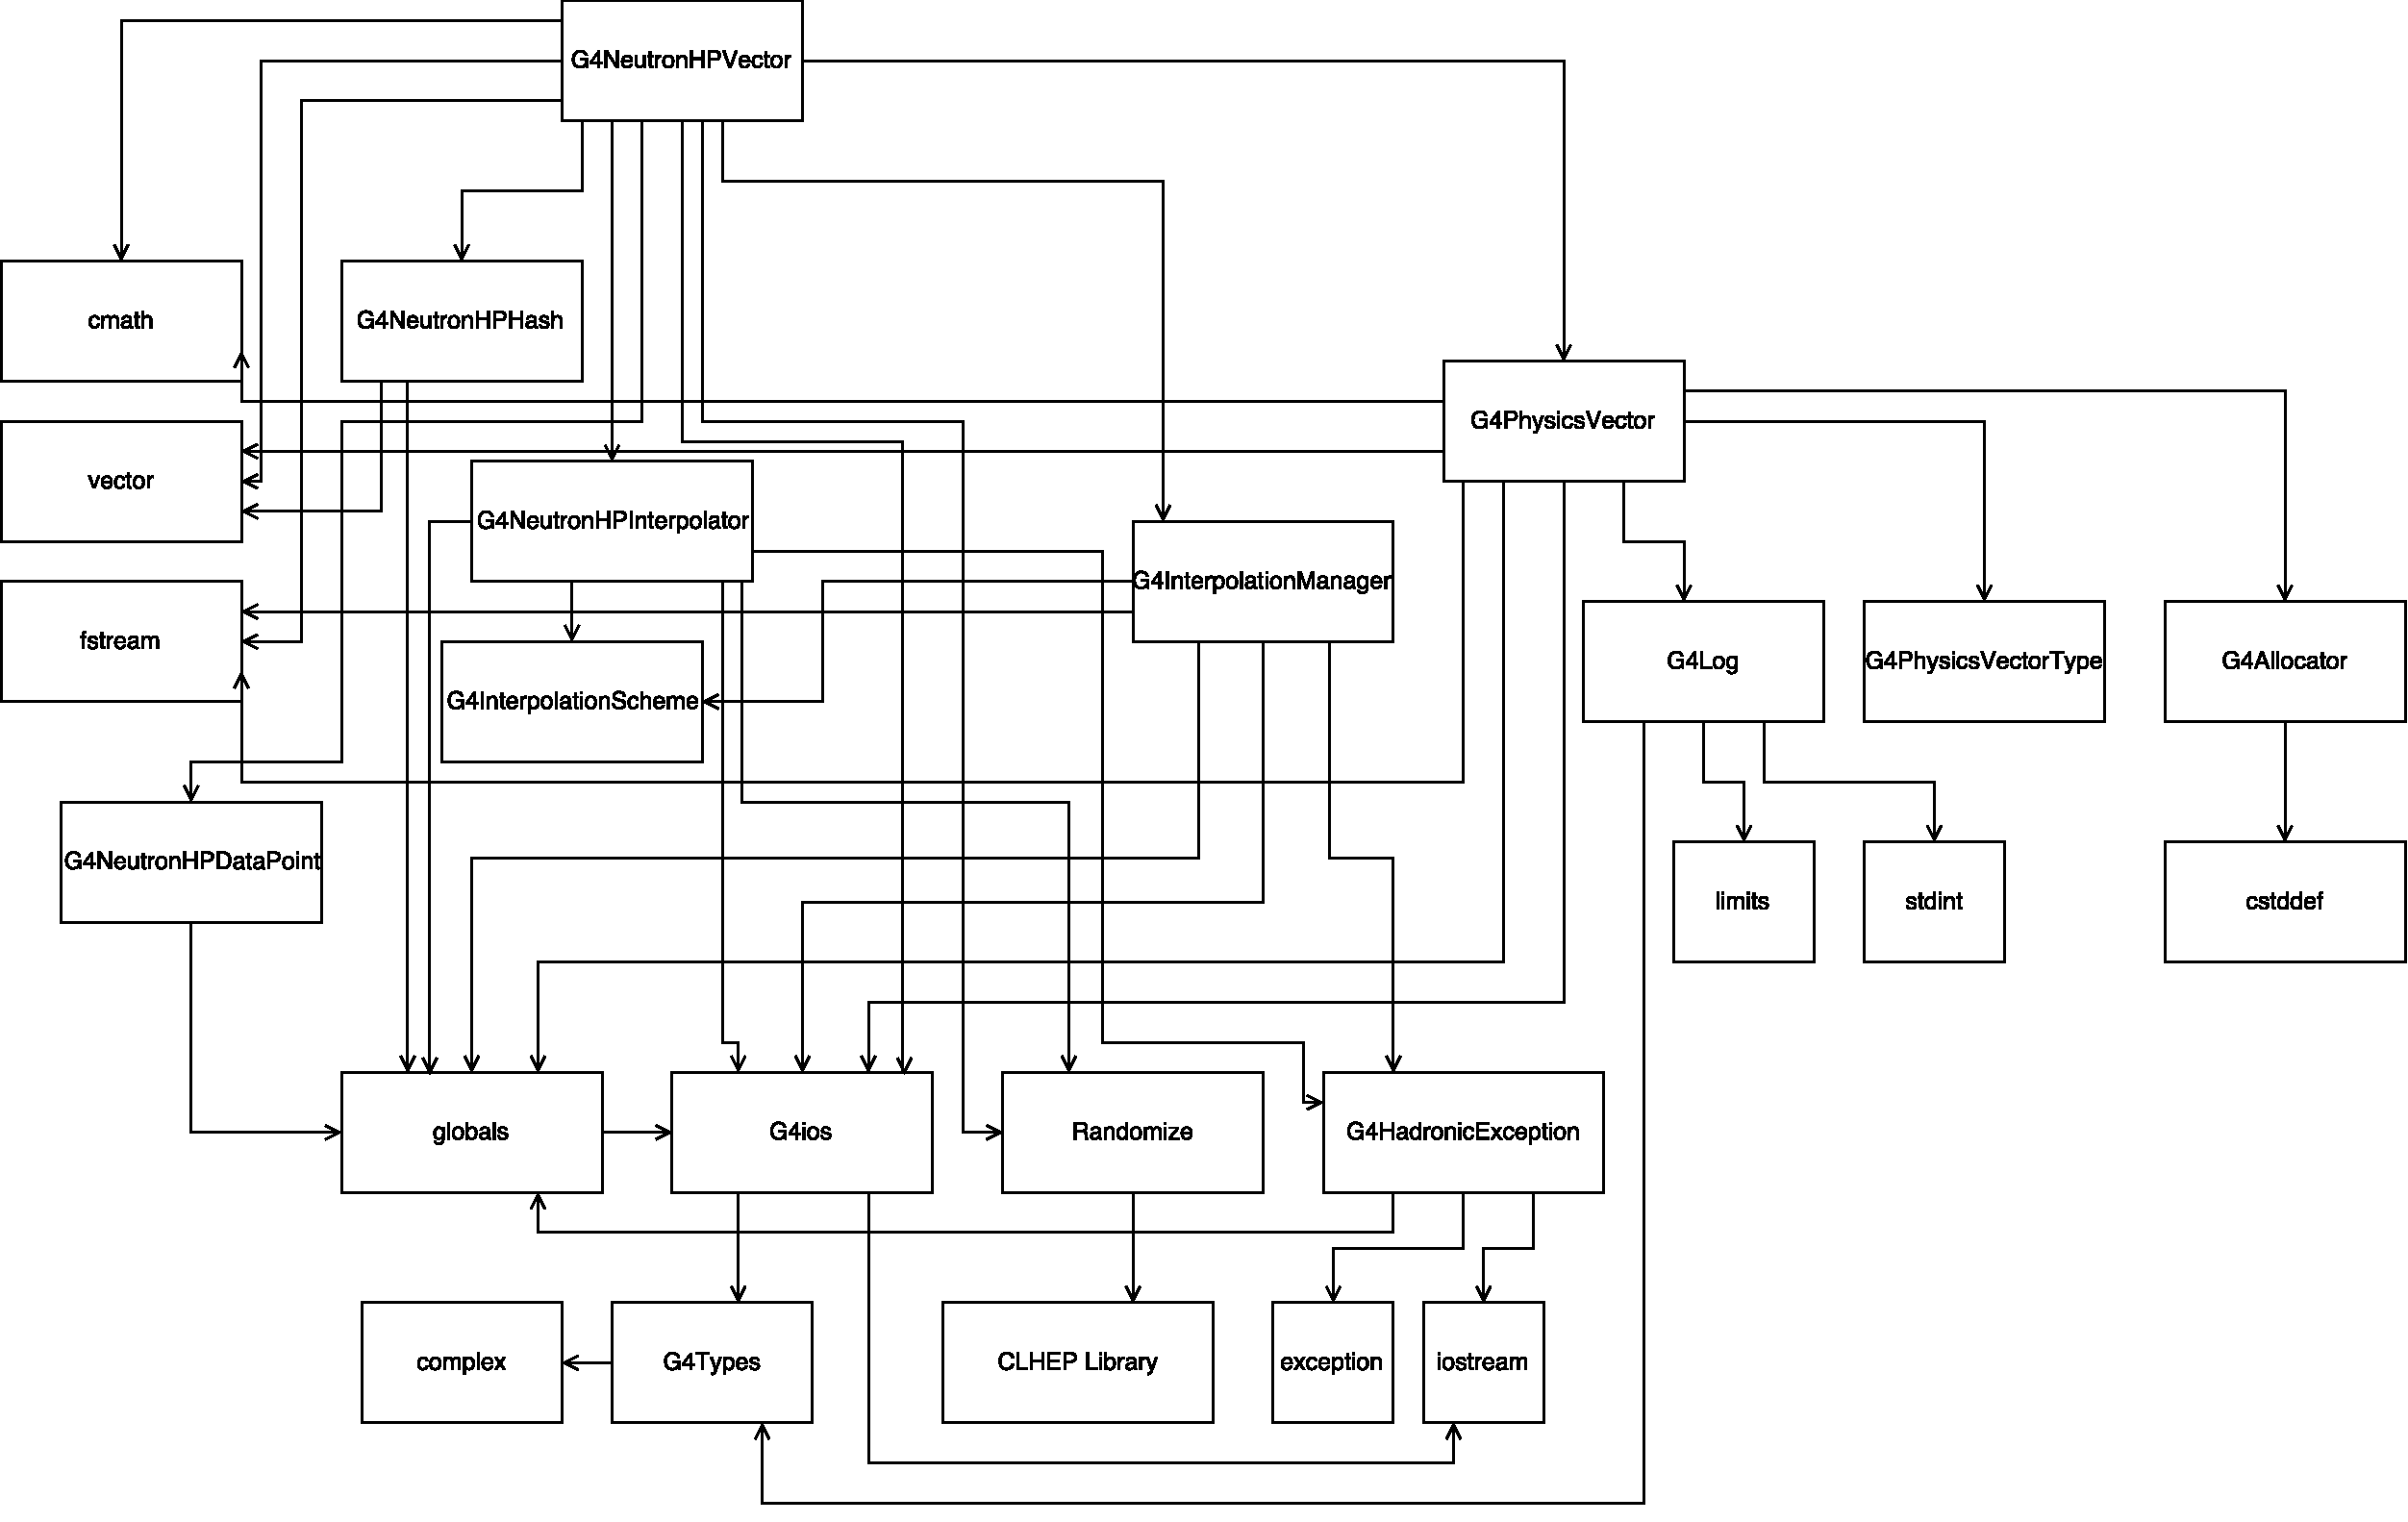
\includegraphics[width=\textwidth]{uses_hierarchy.pdf}
\end{figure}

\section{Traceability of Requirements and Design Components}% ===== Stuart
The following section outlines each requirement and what section of the design document addresses it.

\begin{table}[h]
\centering
\caption{Requirements and Design Relationship}\label{Table_RequirementsAndDesign}
\begin{tabularx}{\textwidth}{cXX}

\toprule
\bf Req. & \bf Brief Description & \bf Design Component\\\midrule
\arrayrulecolor{lightgray}
1  & computations run on GPU & entire document\\\hline
2  & existing projects not affected & \\\hline
3  & by default simulation will run on CPU & \\\hline
4  & should detect if computer has compatible GPU & \\\hline
5  & enabling GPU computation on incompatible hardware not allowed & \\\hline
6  & enabling GPU functionality on existing projects easy & \\\hline
7 & runtime of simulation decreased with same output & \\\hline
8 & accuracy of results same as when run on CPU & \\\hline
9 & at least as stable as existing system & \\\hline
10 & errors will throw exceptions & \\\hline
11 & will work with last four versions of Geant4 & \\\hline
12 & available on public repo with installation instructions & \\\hline
13 & new versions of product will be available on repo, won't break previous features & \\\hline
14 & all users have access to entire product & \\
\arrayrulecolor{black}
\bottomrule
\end{tabularx}
\end{table}

\end{document}
